\documentclass[
  twocolumn,
  aps,
  pra,
  showkeys,
  amsmath,amssymb,
  longbibliography
]{revtex4-2}

\usepackage[T1]{fontenc}
\usepackage[utf8]{inputenc}
\usepackage{mathptmx}
\usepackage{amsthm}
\usepackage{graphicx}
\usepackage{booktabs}
\usepackage{xcolor}
\usepackage{array}
\usepackage{tikz}
\usetikzlibrary{calc,matrix,positioning,decorations.pathreplacing}
\usepackage{alltt}
\usepackage[
  breaklinks=true,
  colorlinks=true,
  citecolor=blue,
  linkcolor=blue,
  urlcolor=blue
]{hyperref}

\newtheorem{proposition}{Proposition}
\newtheorem{definition}{Definition}

% === Eight note colors ===
\definecolor{noteI}{HTML}{3A9D5D}    % C  = green
\definecolor{noteII}{HTML}{3C74C6}   % D  = blue
\definecolor{noteIII}{HTML}{C84332}  % E  = red
\definecolor{noteIV}{HTML}{D8922C}   % F  = orange
\definecolor{noteV}{HTML}{7C52B8}    % G  = violet
\definecolor{noteVI}{HTML}{17BECF}   % A  = teal
\definecolor{noteVII}{HTML}{C44E7D}  % B  = rose
\definecolor{noteVIII}{HTML}{D4AA00} % C2 = gold

% === TikZ tile styles ===
\tikzset{
  pcell/.style={minimum width=3.6mm, minimum height=3.6mm,
                inner sep=0pt, draw=gray!50},
  pone/.style={pcell, fill=black},
  pzero/.style={pcell, fill=white},
  % sequence tiles (slightly larger)
  stile/.style={minimum width=4.2mm, minimum height=4.2mm,
                inner sep=0pt, draw=black!30},
  n1/.style={stile, fill=noteI},
  n2/.style={stile, fill=noteII},
  n3/.style={stile, fill=noteIII},
  n4/.style={stile, fill=noteIV},
  n5/.style={stile, fill=noteV},
  n6/.style={stile, fill=noteVI},
  n7/.style={stile, fill=noteVII},
  n8/.style={stile, fill=noteVIII},
  nsep/.style={stile, fill=black}
}

% === Inline color squares for captions ===
\newcommand{\csq}[1]{%
  {\setlength{\fboxsep}{0pt}%
   \fcolorbox{black}{#1}{\rule{0pt}{1.3ex}\rule{1.3ex}{0pt}}}%
}

% === Color legend ===
\newcommand{\colorlegend}{%
  \csq{noteI}\,C,\;
  \csq{noteII}\,D,\;
  \csq{noteIII}\,E,\;
  \csq{noteIV}\,F,\;
  \csq{noteV}\,G,\;
  \csq{noteVI}\,A,\;
  \csq{noteVII}\,B,\;
  \csq{noteVIII}\,C$_2$%
}

% === Simple listing replacement ===
\newcounter{listing}
\renewcommand{\thelisting}{\arabic{listing}}
\newcommand{\listingtitle}[2]{%
  \refstepcounter{listing}%
  \par\smallskip
  \noindent\textbf{Listing \thelisting.} #2%
  \label{#1}%
  \par\smallskip
}
\newenvironment{codeblock}
  {\par\smallskip\noindent\hrule\smallskip
   \begingroup\footnotesize\ttfamily\begin{alltt}}
  {\end{alltt}\endgroup\smallskip\hrule\smallskip}


\begin{document}

\title{Permutation Matrices as Generative Scores:\\
Noise Models, Minimal Music, and Logic Programming}

\author{Christian Jendreiko}
\affiliation{HSD University of Applied Sciences,
  M\"unsterstra{\ss}e 156, D-40476 D\"usseldorf, Germany}
\email{christian.jendreiko@hs-duesseldorf.de}
\author{Karl Svozil}
\affiliation{Institute for Theoretical Physics, TU Wien,
  Wiedner Hauptstrasse 8-10/136, A-1040 Vienna, Austria}
\email{karl.svozil@tuwien.ac.at}

\date{\today}

\begin{abstract}
We connect the algebraic structure of finite permutation
matrices with Generative Logic by translating sequences of
permutations into Prolog-based Simple Generative Logic
Grammars (SGLGs).
Permutation matrices are motivated as the ``binary
distillation'' of unitary quantum evolution: they retain the
norm-preserving and invertible character of unitary operators
while restricting all matrix entries to~$\{0,1\}$.
As a proof of concept, we use finite permutation matrices of
rank $k=8$ to generate structured sonic artifacts.
By varying the choice of subsequent permutations, we explore
three generative regimes:
``white noise'' (uncorrelated random permutations),
``brown and pink noise'' (random walks and fractal scaling on
the Cayley graph), and
``minimal music'' trajectories (gradually reaching an arbitrary
permutation of rank~$k$ through iterative transpositions in
two-dimensional subspaces).
The approach separates the algebraic progression from its
sonic realization, highlighting the utility of permutation
groups as formal resources for algorithmic composition and
generative design.
\end{abstract}

\keywords{permutation matrices, unitary matrices, orthogonal matrices,
logic programming, generative logic,
algorithmic composition, noise models, minimal music, prolog,
generative art, symmetric group, sound synthesis, quantum mechanics}

\maketitle

%===================================================================
\section{Introduction}
\label{sec:intro}
%===================================================================

This paper connects algebraic combinatorics with algorithmic
composition through the framework of Generative
Logic~\cite{Jendreiko2024,Jendreiko2025}.
While earlier work demonstrated how finite partition logics
can function as generative skeletons for visual
artifacts~\cite{jendreiko-svozil-2026}, the present work
investigates the \emph{dynamic sequencing} of states.
We ask whether sequences of finite permutation matrices can
serve as structural engines for sound generation.

A key motivation comes from quantum mechanics.
The time evolution of a closed quantum system is governed by
\emph{unitary} operators---complex matrices $U$ satisfying
$U^\dagger U=I$---which preserve inner products and
probabilities~\cite{vonneumann-32,peres-93}.
Permutation matrices are the most elementary instances of
unitary operators: they are unitary matrices whose entries are
restricted to the binary set $\{0,1\}$ rather than the full
complex numbers.
In this sense, a permutation matrix is a ``binary
distillation'' of a unitary transformation, retaining the
structural core---invertibility, norm preservation, and
deterministic one-to-one mapping---while discarding all phase
and amplitude freedom.
Intermediate between permutations and full unitaries lie the
\emph{orthogonal} matrices (real entries, $O^{\mathsf T}O=I$),
which preserve real inner products but allow continuous
rotations and reflections.
The resulting group-theoretic hierarchy,
\begin{equation}
S_k \;\subset\; O(k) \;\subset\; U(k),
\label{eq:hierarchy}
\end{equation}
means that every generative idea developed here for the finite
group $S_k$ has a natural continuous generalization to
orthogonal and unitary trajectories.

In algorithmic composition, rule systems have long been used
to constrain or generate sonic material---from Mozart's
\emph{Musikalisches W\"urfelspiel} to the stochastic music of
Iannis Xenakis~\cite{xenakis-71} and the algorithmic phase
shifting of minimalist composers like Steve Reich and Philip
Glass. A particularly close historical precedent is Josef Matthias
Hauer's \emph{Zw\"olftonspiel}~\cite{hauer-25}, which treats
composition as the systematic permutation of twelve pitch
classes within a trope constraint---an approach that we
revisit and generalize in Sec.~\ref{sec:hauer}.

Here, we formalize this generative practice using Prolog and
finite symmetric groups.
A sequence of permutation matrices operates on an initial
vector of sonic events (e.g., an 8-note scale), rearranging it
over time.

The aesthetic character of the generated sound depends
entirely on the \emph{trajectory} taken through the
permutation space.
We systematically construct three distinct categories of
generative scores:
\begin{enumerate}
\item \emph{White noise permutations}: unconstrained, purely
      random selections from~$S_k$.
\item \emph{Brown and pink noise permutations}: structurally
      correlated selections akin to random walks and fractal
      processes on the Cayley graph of~$S_k$.
\item \emph{Minimal music permutations}: deterministic,
      incremental phase-shifting processes that reach a global
      target via minimal rank-2 permutations (acting in
      two-dimensional subspaces).
\end{enumerate}

By framing these concepts within a Simple Generative Logic
Grammar (SGLG)~\cite{Jendreiko2025}, we achieve a clean
separation between the mathematical structure (the permutation
sequence) and the rendering map (the concrete synthesis of
sound), following the three-layer architecture advocated in
Ref.~\cite{jendreiko-svozil-2026}.

%===================================================================
\section{Permutation matrices as generative skeletons}
\label{sec:perm}
%===================================================================

\subsection{Formal structure}

Let $\Omega_k=\{1,2,\ldots,k\}$ be a finite set.
A \emph{permutation} $\pi$ of $\Omega_k$ is a bijection from
the set to itself, belonging to the symmetric group~$S_k$.
This bijection is faithfully represented by a $k\times k$
\emph{permutation matrix}~$P_\sigma$ with entries
\begin{equation}
(P_\sigma)_{ij} = \delta_{j,\,\sigma(i)}.
\label{eq:permmat}
\end{equation}
Every row and column contains exactly one~$1$; all other
entries are~$0$.
The set of all $k\times k$ permutation matrices forms a group
under matrix multiplication isomorphic to~$S_k$, of
order~$k!$ (for $k=8$: $8!=40\,320$).

The action of $P_\sigma$ on a column vector
$\mathbf{v}=(v_1,\ldots,v_k)^{\mathsf T}$ produces
$\mathbf{v}'=P_\sigma\mathbf{v}$, reordering the entries
of~$\mathbf{v}$ according to~$\sigma$.
For artistic generation, $\mathbf{v}$ represents a palette of
media events.
We choose $k=8$, corresponding to a diatonic octave:
\begin{equation}
\mathbf{v}_C = (C,D,E,F,G,A,B,C_2)^{\mathsf T}.
\label{eq:basevec}
\end{equation}
The base vector is visualized as a row of colored tiles in
Fig.~\ref{fig:base}; these eight colors recur in all
subsequent figures.

\begin{figure}[t]
\centering
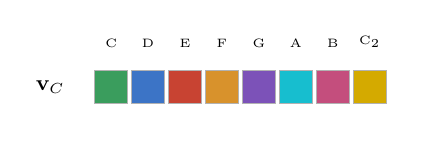
\begin{tikzpicture}[scale=0.88, transform shape]
\matrix (b) [matrix of nodes, nodes in empty cells,
  row sep=1pt, column sep=1pt,
  ampersand replacement=\&] {
|[n1]| \& |[n2]| \& |[n3]| \& |[n4]|
\& |[n5]| \& |[n6]| \& |[n7]| \& |[n8]| \\
};
\node[above=2mm of b-1-1] {\tiny C};
\node[above=2mm of b-1-2] {\tiny D};
\node[above=2mm of b-1-3] {\tiny E};
\node[above=2mm of b-1-4] {\tiny F};
\node[above=2mm of b-1-5] {\tiny G};
\node[above=2mm of b-1-6] {\tiny A};
\node[above=2mm of b-1-7] {\tiny B};
\node[above=2mm of b-1-8] {\tiny C$_2$};
\node[left=3mm of b-1-1] {\small $\mathbf{v}_C$};
\end{tikzpicture}
\caption{The base vector $\mathbf{v}_C$ rendered as eight
colored tiles.
Color key used throughout:
\colorlegend.}
\label{fig:base}
\end{figure}

\subsection{Quantum-mechanical motivation: from unitary to
permutation matrices}
\label{sec:qm}

The choice of permutation matrices as primary generative
entities is not arbitrary; it is rooted in the mathematical
framework of quantum mechanics.

In quantum theory, the time evolution of a closed system with
a $k$-dimensional state space is described by a $k\times k$
\emph{unitary matrix}~$U$, i.e., a matrix with complex entries
satisfying~\cite{vonneumann-32,peres-93}
\begin{equation}
U^\dagger U = U U^\dagger = I,
\label{eq:unitary}
\end{equation}
where $U^\dagger$ denotes the conjugate transpose.
Unitarity guarantees that the transformation is invertible,
that it preserves the inner product
$\langle\psi|\phi\rangle$, and hence that all probabilities
and norms are conserved.
The set of all such matrices forms the \emph{unitary group}
$U(k)$, a continuous Lie group of (real)
dimension~$k^2$~\cite{hall-15}.

If one restricts attention to matrices with purely \emph{real}
entries, the unitarity condition $U^\dagger U=I$ reduces to
orthogonality:
\begin{equation}
O^{\mathsf T} O = O O^{\mathsf T} = I,
\qquad O_{ij}\in\mathbb{R}.
\label{eq:orthogonal}
\end{equation}
These \emph{orthogonal matrices} form the orthogonal group
$O(k)\subset U(k)$, of dimension $k(k-1)/2$.
Orthogonal transformations preserve real inner products and
include rotations and reflections in $\mathbb{R}^k$.

If one further restricts the matrix entries from the reals to
the binary set $\{0,1\}$, while still requiring that each row
and each column contain exactly one nonzero entry, one obtains
precisely the \emph{permutation matrices}.
Every permutation matrix is trivially orthogonal (and hence
unitary), since its columns form an orthonormal set with
respect to both the real and the complex inner product.
But whereas $U(k)$ and $O(k)$ are continuous groups of
infinite cardinality, the permutation matrices form the
\emph{finite} symmetric group $S_k$ of order~$k!$.

This yields the nested inclusion chain already stated in
Eq.~\eqref{eq:hierarchy}:
\begin{equation}
S_k \;\subset\; O(k) \;\subset\; U(k).
\label{eq:hierarchy2}
\end{equation}

Table~\ref{tab:hierarchy} summarizes the three levels.
Moving upward in the hierarchy, one trades finiteness and
combinatorial transparency for continuous phase freedom and
richer interference effects.
Moving downward, one distills the essential structural
properties of unitary evolution---invertibility, norm
preservation, one-to-one mapping of basis
states---into a finite, combinatorial object.

\begin{table}[b]
\caption{The hierarchy from unitary to permutation matrices.
Each level preserves inner products and is invertible;
the levels differ in the number field and the size of the
resulting group.}
\label{tab:hierarchy}
\begin{ruledtabular}
\begin{tabular}{lccc}
Group & Entries & Dimension & Size \\
\hline
$U(k)$ & $\mathbb{C}$   & $k^2$ & $\infty$ (Lie) \\
$O(k)$ & $\mathbb{R}$   & $k(k{-}1)/2$ & $\infty$ (Lie) \\
$S_k$  & $\{0,1\}$      & $0$ (discrete) & $k!$ \\
\end{tabular}
\end{ruledtabular}
\end{table}

This perspective clarifies why permutation matrices are a
natural starting point for generative exploration.
They are the \emph{simplest nontrivial unitary operators}:
they shuffle basis vectors without introducing any relative
phases or superpositions.
In quantum-information language, permutation matrices
correspond to \emph{classical reversible gates} acting on
computational basis states~\cite{nielsen-chuang-00}.
They are exactly the unitary operators that map every
computational basis state to another computational basis
state, never creating superpositions.

The Birkhoff--von Neumann theorem~\cite{birkhoff-46}
provides a further structural link: every \emph{doubly
stochastic} matrix (i.e., a nonnegative matrix whose rows and
columns each sum to~$1$) can be written as a convex
combination of permutation matrices.
Since the modulus-squared entries of any unitary matrix, taken
row-by-row or column-by-column, form a doubly stochastic
matrix~\cite{schur-23,horn-54}, permutation matrices are the
extreme points of the polytope that bounds all
quantum-mechanically admissible probability tables.

For the generative framework of this paper, the key
consequence is methodological.
Every construction we develop for permutation
sequences---white, brown, pink, and minimal-music
regimes---can in principle be lifted to orthogonal or unitary
trajectories, replacing the discrete Cayley graph of $S_k$ by
geodesics, Brownian motion, or fractional processes on $O(k)$
or~$U(k)$~\cite{liao-04}.
The permutation-matrix case is the ``binary skeleton'' of such
continuous constructions: it captures the combinatorial
essence while remaining finite, explicit, and implementable in
a logic-programming environment.

A concrete illustration of the distillation is provided by the
rank-2 case.
A general $2\times 2$ unitary matrix can be parameterized
(up to a global phase) as
\begin{equation}
U_2(\theta,\phi,\lambda) =
\begin{pmatrix}
\cos\theta & -e^{i\lambda}\sin\theta \\
e^{i\phi}\sin\theta & e^{i(\phi+\lambda)}\cos\theta
\end{pmatrix}.
\label{eq:u2}
\end{equation}
Restricting to real entries ($\phi=\lambda=0$) yields the
$2\times 2$ rotation (orthogonal) matrix
\begin{equation}
O_2(\theta) =
\begin{pmatrix}
\cos\theta & -\sin\theta \\
\sin\theta & \cos\theta
\end{pmatrix}.
\label{eq:o2}
\end{equation}
Further restricting to $\{0,1\}$ entries leaves only two
possibilities: the identity ($\theta=0$) and the swap
\begin{equation}
P_{\tau_{12}} =
\begin{pmatrix}
0 & 1 \\
1 & 0
\end{pmatrix},
\label{eq:swap2}
\end{equation}
which is the unique nontrivial $2\times 2$ permutation
matrix---our rank-2 transposition.
The continuous rotation family~\eqref{eq:o2} interpolates
smoothly between identity and swap; the permutation matrix
retains only the two endpoints.
This is the sense in which permutations are the ``binary
distillation'' of unitary (or orthogonal) transformations.

\subsection{Transpositions and rank-2 permutations}

Every $\sigma\in S_k$ can be written as a product of
\emph{transpositions} $\tau_{ij}$, each swapping elements
$i$ and~$j$.
In matrix terms, $P_{\tau_{ij}}$ differs from the identity only
in a $2\times 2$ block acting on the span of the $i$ and $j$ basis vectors,
exactly as in Eq.~\eqref{eq:swap2} (if $i$ and $j$ are adjacent, it is literally a contiguous $2\times 2$ block).
We call it a \emph{rank-2 permutation matrix} because it acts
nontrivially only on a two-dimensional subspace---the
permutation-matrix analogue of a Givens
rotation~\cite{golub-vanloan-13} in numerical linear algebra.
Every $\sigma\in S_k$ can be decomposed into at most $k-1$
transpositions; if one insists on \emph{adjacent}
transpositions $\tau_{i,i+1}$, the minimum number needed is
the Kendall tau distance (number of inversions).

\subsection{Concrete example}

Consider $\pi=(1\;3\;5\;7)(2\;4\;6\;8)\in S_8$,
which maps $1\!\to\!3$, $3\!\to\!5$, $5\!\to\!7$,
$7\!\to\!1$, $2\!\to\!4$, $4\!\to\!6$, $6\!\to\!8$,
$8\!\to\!2$.
As a list: $\sigma=[3,4,5,6,7,8,1,2]$.
Figure~\ref{fig:exampleperm}(a) shows the $8\times 8$
permutation matrix; panel~(b) shows the result
$P_\sigma\mathbf{v}_C$: the eight notes have been cyclically
shifted in two interlocking quartets.

\begin{figure}[t]
\centering
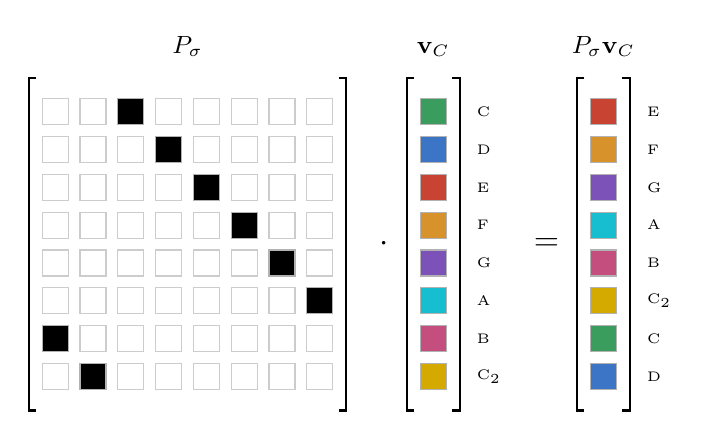
\begin{tikzpicture}[
  scale=2,
  x=2.4mm, y=2.4mm,
  mone/.style={fill=black, draw=gray!60,
    minimum size=3.3mm, inner sep=0pt},
  mzero/.style={fill=white, draw=gray!40,
    minimum size=3.3mm, inner sep=0pt},
  vc/.style={fill=#1, draw=black!30,
    minimum size=3.3mm, inner sep=0pt}
]

% ========== Permutation matrix P_sigma ==========
\def\perm{{3,4,5,6,7,8,1,2}}
\foreach \i in {0,...,7}{
  \foreach \j in {0,...,7}{
    \pgfmathtruncatemacro{\val}{\perm[\i]==(\j+1)?1:0}
    \ifnum\val=1
      \node[mone] at (\j+0.5, -\i-0.5) {};
    \else
      \node[mzero] at (\j+0.5, -\i-0.5) {};
    \fi
  }
}
% Left bracket
\draw[thick] (0, 0.4) -- (-0.2, 0.4)
  -- (-0.2, -8.4) -- (0, -8.4);
% Right bracket
\draw[thick] (8, 0.4) -- (8.2, 0.4)
  -- (8.2, -8.4) -- (8, -8.4);
% Label
\node[above] at (4, 0.7) {\small $P_\sigma$};

% ========== Multiplication dot ==========
\node at (9.2, -4) {\large $\cdot$};

% ========== Input vector v_C ==========
\node[vc=noteI]    at (10.5, -0.5) {};
\node[vc=noteII]   at (10.5, -1.5) {};
\node[vc=noteIII]  at (10.5, -2.5) {};
\node[vc=noteIV]   at (10.5, -3.5) {};
\node[vc=noteV]    at (10.5, -4.5) {};
\node[vc=noteVI]   at (10.5, -5.5) {};
\node[vc=noteVII]  at (10.5, -6.5) {};
\node[vc=noteVIII] at (10.5, -7.5) {};
% Left bracket
\draw[thick] (10, 0.4) -- (9.8, 0.4)
  -- (9.8, -8.4) -- (10, -8.4);
% Right bracket
\draw[thick] (11, 0.4) -- (11.2, 0.4)
  -- (11.2, -8.4) -- (11, -8.4);
% Label
\node[above] at (10.5, 0.7) {\small $\mathbf{v}_C$};
% Note labels
\node[right, font=\tiny] at (11.4, -0.5) {C};
\node[right, font=\tiny] at (11.4, -1.5) {D};
\node[right, font=\tiny] at (11.4, -2.5) {E};
\node[right, font=\tiny] at (11.4, -3.5) {F};
\node[right, font=\tiny] at (11.4, -4.5) {G};
\node[right, font=\tiny] at (11.4, -5.5) {A};
\node[right, font=\tiny] at (11.4, -6.5) {B};
\node[right, font=\tiny] at (11.4, -7.5) {C$_2$};

% ========== Equals sign ==========
\node at (13.5, -4) {\large $=$};

% ========== Output vector P_sigma v_C ==========
% sigma=[3,4,5,6,7,8,1,2] -> E,F,G,A,B,C2,C,D
\node[vc=noteIII]  at (15, -0.5) {};
\node[vc=noteIV]   at (15, -1.5) {};
\node[vc=noteV]    at (15, -2.5) {};
\node[vc=noteVI]   at (15, -3.5) {};
\node[vc=noteVII]  at (15, -4.5) {};
\node[vc=noteVIII] at (15, -5.5) {};
\node[vc=noteI]    at (15, -6.5) {};
\node[vc=noteII]   at (15, -7.5) {};
% Left bracket
\draw[thick] (14.5, 0.4) -- (14.3, 0.4)
  -- (14.3, -8.4) -- (14.5, -8.4);
% Right bracket
\draw[thick] (15.5, 0.4) -- (15.7, 0.4)
  -- (15.7, -8.4) -- (15.5, -8.4);
% Label
\node[above] at (15, 0.7)
  {\small $P_\sigma\mathbf{v}_C$};
% Note labels
\node[right, font=\tiny] at (15.9, -0.5) {E};
\node[right, font=\tiny] at (15.9, -1.5) {F};
\node[right, font=\tiny] at (15.9, -2.5) {G};
\node[right, font=\tiny] at (15.9, -3.5) {A};
\node[right, font=\tiny] at (15.9, -4.5) {B};
\node[right, font=\tiny] at (15.9, -5.5) {C$_2$};
\node[right, font=\tiny] at (15.9, -6.5) {C};
\node[right, font=\tiny] at (15.9, -7.5) {D};

\end{tikzpicture}
\caption{The matrix equation
$P_\sigma\,\mathbf{v}_C = \mathbf{v}'$ for
$\sigma=(1\;3\;5\;7)(2\;4\;6\;8)\in S_8$.
The $8\times 8$ permutation matrix
(black cells${}\!=\!1$, white cells${}\!=\!0$) acts on the
color-coded base vector
$\mathbf{v}_C=(C,D,E,F,G,A,B,C_2)^{\mathsf T}$,
producing the output
$\mathbf{v}'=(E,F,G,A,B,C_2,C,D)^{\mathsf T}$.
Colors as in Fig.~\ref{fig:base}.}
\label{fig:exampleperm}
\end{figure}

When a \emph{sequence} of permutation matrices
$P_1,P_2,\ldots,P_N$ is applied iteratively to
$\mathbf{v}_C$, it generates a score of length~$N$: each
``row'' is a rearrangement of the eight base notes.
How the sequence $\{P_t\}$ is selected dictates the
``logic'' of the musical composition.

%===================================================================
\section{White noise permutations}
\label{sec:white}
%===================================================================

A \emph{white noise} sequence is generated by selecting each
$P_t$ independently and uniformly at random from~$S_k$:
\begin{equation}
P_t \sim \mathcal{U}(S_k).
\label{eq:white}
\end{equation}
Algorithmically, a uniformly random permutation is produced by
the Fisher--Yates shuffle~\cite{knuth-97}.

In a musical context, this sequence lacks memory.
Every step results in a complete reshuffling of the tonal
material.
Because the expected distance between $P_t$ and $P_{t+1}$ on
the Cayley graph is near-maximal (a random permutation fixes
on average only one element~\cite{knuth-97}), the resulting
sound texture is chaotic and saturated.

In the quantum-mechanical analogy of
Sec.~\ref{sec:qm}, this regime corresponds to applying a
sequence of independently Haar-random unitary
matrices~\cite{mezzadri-07}---the unitary analogue of white
noise---but distilled to the binary $\{0,1\}$ skeleton of
$S_k$.

\paragraph*{Concrete example.}
Six successive random permutations of rank~$8$ and their
color renderings are shown in Fig.~\ref{fig:white}.
Note the complete lack of column-wise continuity: every color
appears at unpredictable positions from row to row.

\begin{figure}[t]
\centering
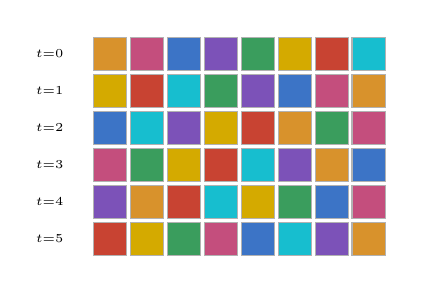
\begin{tikzpicture}[scale=0.88, transform shape]
\matrix (w) [matrix of nodes, nodes in empty cells,
  row sep=1pt, column sep=1pt,
  ampersand replacement=\&] {
|[n4]| \& |[n7]| \& |[n2]| \& |[n5]|
\& |[n1]| \& |[n8]| \& |[n3]| \& |[n6]| \\
|[n8]| \& |[n3]| \& |[n6]| \& |[n1]|
\& |[n5]| \& |[n2]| \& |[n7]| \& |[n4]| \\
|[n2]| \& |[n6]| \& |[n5]| \& |[n8]|
\& |[n3]| \& |[n4]| \& |[n1]| \& |[n7]| \\
|[n7]| \& |[n1]| \& |[n8]| \& |[n3]|
\& |[n6]| \& |[n5]| \& |[n4]| \& |[n2]| \\
|[n5]| \& |[n4]| \& |[n3]| \& |[n6]|
\& |[n8]| \& |[n1]| \& |[n2]| \& |[n7]| \\
|[n3]| \& |[n8]| \& |[n1]| \& |[n7]|
\& |[n2]| \& |[n6]| \& |[n5]| \& |[n4]| \\
};
\node[left=3mm of w-1-1] {\tiny $t{=}0$};
\node[left=3mm of w-2-1] {\tiny $t{=}1$};
\node[left=3mm of w-3-1] {\tiny $t{=}2$};
\node[left=3mm of w-4-1] {\tiny $t{=}3$};
\node[left=3mm of w-5-1] {\tiny $t{=}4$};
\node[left=3mm of w-6-1] {\tiny $t{=}5$};
\end{tikzpicture}
\caption{\textbf{White noise}: six successive uniformly random
permutations of rank~$8$, rendered as colored tile rows.
Each row is a complete rearrangement of
$\mathbf{v}_C$; no column shows temporal continuity.
Colors as in Fig.~\ref{fig:base}.}
\label{fig:white}
\end{figure}

%===================================================================
\section{Brown noise permutations}
\label{sec:brown}
%===================================================================

\emph{Brown noise} (Brownian noise) in signal processing is
generated by integrating white noise.
In permutation space, this corresponds to a random walk on the
Cayley graph of~$S_k$ with respect to adjacent
transpositions~\cite{diaconis-shahshahani-81}:
\begin{equation}
P_{t+1} = P_t\;\tau_{i_t,\,i_t+1},
\qquad
i_t\sim\mathrm{Uniform}\{1,\ldots,k{-}1\}.
\label{eq:brown}
\end{equation}
Each step changes at most two voice assignments by one scale
degree, so the spectral density of each voice's pitch
trajectory goes as~$1/f^2$.

In the unitary hierarchy~\eqref{eq:hierarchy2}, the
continuous analogue is Brownian motion on $O(k)$ or $U(k)$,
generated by infinitesimal rotations drawn from the Lie
algebra~\cite{liao-04}.
The permutation random walk is the binary skeleton of this
process: the Lie-algebra generators (skew-symmetric matrices
with continuous entries) are replaced by adjacent
transpositions (the simplest generators of~$S_k$).

\paragraph*{Concrete example.}
Starting from the identity, a sample random walk of eight
steps is shown in Fig.~\ref{fig:brown}.
At each step exactly one adjacent pair of tiles is swapped.
The visual impression is one of slow drift: most columns
retain their color across several time steps.

\begin{figure}[t]
\centering
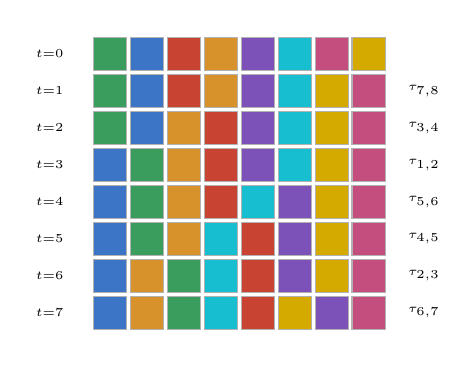
\begin{tikzpicture}[scale=0.88, transform shape]
\matrix (br) [matrix of nodes, nodes in empty cells,
  row sep=1pt, column sep=1pt,
  ampersand replacement=\&] {
|[n1]| \& |[n2]| \& |[n3]| \& |[n4]|
\& |[n5]| \& |[n6]| \& |[n7]| \& |[n8]| \\
|[n1]| \& |[n2]| \& |[n3]| \& |[n4]|
\& |[n5]| \& |[n6]| \& |[n8]| \& |[n7]| \\
|[n1]| \& |[n2]| \& |[n4]| \& |[n3]|
\& |[n5]| \& |[n6]| \& |[n8]| \& |[n7]| \\
|[n2]| \& |[n1]| \& |[n4]| \& |[n3]|
\& |[n5]| \& |[n6]| \& |[n8]| \& |[n7]| \\
|[n2]| \& |[n1]| \& |[n4]| \& |[n3]|
\& |[n6]| \& |[n5]| \& |[n8]| \& |[n7]| \\
|[n2]| \& |[n1]| \& |[n4]| \& |[n6]|
\& |[n3]| \& |[n5]| \& |[n8]| \& |[n7]| \\
|[n2]| \& |[n4]| \& |[n1]| \& |[n6]|
\& |[n3]| \& |[n5]| \& |[n8]| \& |[n7]| \\
|[n2]| \& |[n4]| \& |[n1]| \& |[n6]|
\& |[n3]| \& |[n8]| \& |[n5]| \& |[n7]| \\
};
\node[left=3mm of br-1-1] {\tiny $t{=}0$};
\node[left=3mm of br-2-1] {\tiny $t{=}1$};
\node[left=3mm of br-3-1] {\tiny $t{=}2$};
\node[left=3mm of br-4-1] {\tiny $t{=}3$};
\node[left=3mm of br-5-1] {\tiny $t{=}4$};
\node[left=3mm of br-6-1] {\tiny $t{=}5$};
\node[left=3mm of br-7-1] {\tiny $t{=}6$};
\node[left=3mm of br-8-1] {\tiny $t{=}7$};
\node[right=2mm of br-2-8] {\tiny $\tau_{7,8}$};
\node[right=2mm of br-3-8] {\tiny $\tau_{3,4}$};
\node[right=2mm of br-4-8] {\tiny $\tau_{1,2}$};
\node[right=2mm of br-5-8] {\tiny $\tau_{5,6}$};
\node[right=2mm of br-6-8] {\tiny $\tau_{4,5}$};
\node[right=2mm of br-7-8] {\tiny $\tau_{2,3}$};
\node[right=2mm of br-8-8] {\tiny $\tau_{6,7}$};
\end{tikzpicture}
\caption{\textbf{Brown noise}: a random walk on $S_8$ via
adjacent transpositions, starting from the identity.
At each step, the applied transposition $\tau_{i,i+1}$ is
annotated on the right.
Most columns show high continuity; changes propagate slowly.}
\label{fig:brown}
\end{figure}

Aesthetically, a Brownian permutation sequence exhibits high
structural continuity.
Each generated row differs from the previous one by exactly
two transposed elements.
The listener perceives a slowly morphing textural field, where
melody lines gradually evolve rather than randomly
jump---reminiscent of the glissando textures in orchestral
works by Xenakis~\cite{xenakis-71}.

The random walk on~$S_k$ is ergodic, with mixing time
$\Theta(k^3\log k)$~\cite{diaconis-shahshahani-81}; for
$k=8$ this is of order~$10^3$ steps.

%===================================================================
\section{Pink noise (fractal) permutations}
\label{sec:pink}
%===================================================================

Pink noise ($1/f$ noise) sits between the chaotic
unpredictability of white noise and the heavy correlation of
brown noise, exhibiting fractal scale
invariance~\cite{voss-clarke-75,voss-clarke-78}.

Direct generation of $1/f$ noise in a group-valued setting is
nontrivial.
We adopt a multi-scale superposition strategy inspired by the
Voss--McCartney algorithm~\cite{voss-clarke-78,gardner-78}:
\begin{enumerate}
\item Maintain $K=\lceil\log_2 k\rceil$ independent
      registers $R_0,\ldots,R_{K-1}$, each holding an
      adjacent transposition.
\item At step~$t$, re-randomize register~$m$ whenever bit~$m$
      of the binary representation of~$t$ changes relative
      to~$t{-}1$.
      Register~$0$ updates every step, register~$1$ every
      two steps, etc.
\item Compose: $P_t = R_{K-1}\circ\cdots\circ R_1\circ R_0$,
      applied to the identity.
\end{enumerate}

In the unitary picture, the analogue would be a product of
$K$ independent Givens rotations at different time scales,
yielding a fractal process on~$O(k)$.
The permutation version discretizes each factor to its two
$\{0,1\}$-extremes: identity or swap.

\paragraph*{Concrete example.}
Using $K=3$ registers with adjacent transpositions, we traced
eight steps explicitly.
The register states and resulting permutations are:

\smallskip
\noindent
\begin{tabular}{@{}cl@{\;}l@{\;}ll@{}}
\toprule
$t$ & $R_0$ & $R_1$ & $R_2$ & Result \\
\midrule
0 & id & id & id & $[1,2,3,4,5,6,7,8]$ \\
1 & $\tau_{3,4}$ & id & id & $[1,2,4,3,5,6,7,8]$ \\
2 & $\tau_{6,7}$ & $\tau_{2,3}$ & id & $[1,3,2,4,5,7,6,8]$ \\
3 & $\tau_{1,2}$ & $\tau_{2,3}$ & id & $[2,3,1,4,5,6,7,8]$ \\
4 & $\tau_{5,6}$ & $\tau_{4,5}$ & $\tau_{7,8}$ & $[1,2,3,6,4,5,8,7]$ \\
5 & $\tau_{2,3}$ & $\tau_{4,5}$ & $\tau_{7,8}$ & $[1,3,2,5,4,6,8,7]$ \\
6 & $\tau_{1,2}$ & $\tau_{3,4}$ & $\tau_{7,8}$ & $[2,1,4,3,5,6,8,7]$ \\
7 & $\tau_{6,7}$ & $\tau_{3,4}$ & $\tau_{7,8}$ & $[1,2,4,3,5,7,8,6]$ \\
\bottomrule
\end{tabular}
\smallskip

\noindent
The color rendering appears in Fig.~\ref{fig:pink}.
At $t=4$, all three registers update simultaneously, producing
the largest visual discontinuity.
Single-register updates ($t=1,3,5,7$) cause smaller changes.
This multi-scale behavior yields a ``musical'' balance of
repetition and surprise.

\begin{figure}[t]
\centering
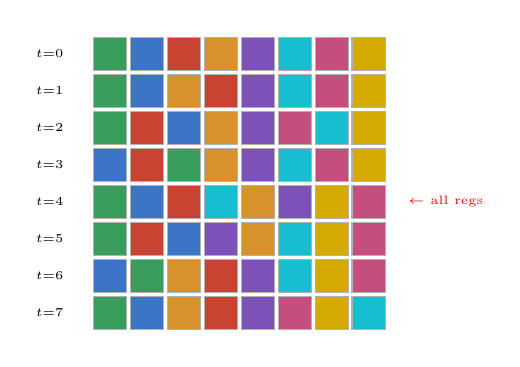
\begin{tikzpicture}[scale=0.88, transform shape]
\matrix (pk) [matrix of nodes, nodes in empty cells,
  row sep=1pt, column sep=1pt,
  ampersand replacement=\&] {
|[n1]| \& |[n2]| \& |[n3]| \& |[n4]|
\& |[n5]| \& |[n6]| \& |[n7]| \& |[n8]| \\
|[n1]| \& |[n2]| \& |[n4]| \& |[n3]|
\& |[n5]| \& |[n6]| \& |[n7]| \& |[n8]| \\
|[n1]| \& |[n3]| \& |[n2]| \& |[n4]|
\& |[n5]| \& |[n7]| \& |[n6]| \& |[n8]| \\
|[n2]| \& |[n3]| \& |[n1]| \& |[n4]|
\& |[n5]| \& |[n6]| \& |[n7]| \& |[n8]| \\
|[n1]| \& |[n2]| \& |[n3]| \& |[n6]|
\& |[n4]| \& |[n5]| \& |[n8]| \& |[n7]| \\
|[n1]| \& |[n3]| \& |[n2]| \& |[n5]|
\& |[n4]| \& |[n6]| \& |[n8]| \& |[n7]| \\
|[n2]| \& |[n1]| \& |[n4]| \& |[n3]|
\& |[n5]| \& |[n6]| \& |[n8]| \& |[n7]| \\
|[n1]| \& |[n2]| \& |[n4]| \& |[n3]|
\& |[n5]| \& |[n7]| \& |[n8]| \& |[n6]| \\
};
\node[left=3mm of pk-1-1] {\tiny $t{=}0$};
\node[left=3mm of pk-2-1] {\tiny $t{=}1$};
\node[left=3mm of pk-3-1] {\tiny $t{=}2$};
\node[left=3mm of pk-4-1] {\tiny $t{=}3$};
\node[left=3mm of pk-5-1] {\tiny $t{=}4$};
\node[left=3mm of pk-6-1] {\tiny $t{=}5$};
\node[left=3mm of pk-7-1] {\tiny $t{=}6$};
\node[left=3mm of pk-8-1] {\tiny $t{=}7$};
\node[right=2mm of pk-5-8]
  {\tiny\color{red}$\leftarrow$ all regs};
\end{tikzpicture}
\caption{\textbf{Pink noise}: eight steps of a
Voss--McCartney permutation sequence with $K=3$
adjacent-transposition registers.
At $t=4$ (arrow), all three registers update, causing a large
rearrangement.
Between major updates the sequence drifts smoothly.}
\label{fig:pink}
\end{figure}

Table~\ref{tab:regimes} compares the three stochastic regimes.

\begin{table}[t]
\caption{Summary of the three noise regimes for permutation
sequences ($k=8$ voices) and their continuous analogues on
$O(k)$ or $U(k)$.}
\label{tab:regimes}
\begin{ruledtabular}
\begin{tabular}{lccl}
Regime & Spectrum & $O(k)/U(k)$ analogue & Character \\
\hline
White  & flat     & Haar-random   & chaotic \\
Brown  & $1/f^2$  & Brownian      & slow drift \\
Pink   & $1/f$    & fractal       & natural flow \\
\end{tabular}
\end{ruledtabular}
\end{table}

%===================================================================
\section{Minimal music and rank-2 permutations}
\label{sec:minimal}
%===================================================================

While the noise models rely on stochastic choices,
\emph{minimal music} (typified by Steve Reich's
\emph{Piano Phase}) is characterized by strictly
deterministic, gradual, and cumulative processes.
We model this using purely algorithmic traversals of~$S_k$.

\begin{proposition}
Any permutation matrix $P$ of rank~$k$ can be reached from
the identity $I$ by a sequence of at most $k-1$ transpositions
acting in two-dimensional subspaces.
\end{proposition}

\begin{proof}
Standard: place elements into their correct positions
sequentially; each placement requires at most one
transposition.
\end{proof}

In the language of the unitary hierarchy, this decomposition
is the discrete analogue of factoring a unitary matrix into a
product of Givens rotations~\cite{golub-vanloan-13} or
two-level unitary matrices~\cite{nielsen-chuang-00}.
In the orthogonal case, any $O\in O(k)$ can be written as a
product of at most $k(k-1)/2$ Givens rotations; the
permutation case collapses each continuous rotation to the
binary choice of ``swap or not.''

To generate a minimal music score, we \emph{sonify the
incremental journey} rather than jumping directly to the
target:
\begin{equation}
P_0 = I,\;
P_1 = T_1,\;
P_2 = T_1 T_2,\;
\ldots,\;
P_m = T_1\cdots T_m = P_{\mathrm{target}},
\label{eq:minpath}
\end{equation}
where each $T_i$ is a rank-2 transposition.
By repeating each state $P_i$ multiple times (ostinato) before
transitioning to $P_{i+1}$, the grammar produces the
characteristic additive structure of minimalist composition.

\paragraph*{Concrete example.}
Let the target be the ``paired swap'' permutation
$\sigma_{\star}=[2,1,4,3,6,5,8,7]$, which exchanges every
adjacent pair.
A minimal decomposition uses four transpositions:
\begin{align}
P_0 &= [1,2,3,4,5,6,7,8], \nonumber\\
P_1 &= [2,1,3,4,5,6,7,8] \quad(\tau_{1,2}), \nonumber\\
P_2 &= [2,1,4,3,5,6,7,8] \quad(\tau_{3,4}), \nonumber\\
P_3 &= [2,1,4,3,6,5,7,8] \quad(\tau_{5,6}), \nonumber\\
P_4 &= [2,1,4,3,6,5,8,7] \quad(\tau_{7,8}).
\label{eq:minex}
\end{align}
Figure~\ref{fig:minimal}(a) shows these five states as tile
rows.
Panel~(b) shows the same path with each state repeated
three times (ostinato), yielding the mesmerizing repetitive
texture characteristic of minimal music.

\begin{figure}[t]
\centering
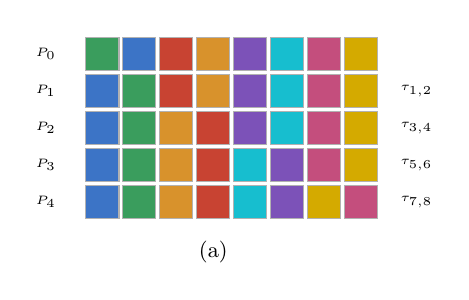
\begin{tikzpicture}[scale=0.88, transform shape]
\matrix (mi) [matrix of nodes, nodes in empty cells,
  row sep=1pt, column sep=1pt,
  ampersand replacement=\&] {
|[n1]| \& |[n2]| \& |[n3]| \& |[n4]|
\& |[n5]| \& |[n6]| \& |[n7]| \& |[n8]| \\
|[n2]| \& |[n1]| \& |[n3]| \& |[n4]|
\& |[n5]| \& |[n6]| \& |[n7]| \& |[n8]| \\
|[n2]| \& |[n1]| \& |[n4]| \& |[n3]|
\& |[n5]| \& |[n6]| \& |[n7]| \& |[n8]| \\
|[n2]| \& |[n1]| \& |[n4]| \& |[n3]|
\& |[n6]| \& |[n5]| \& |[n7]| \& |[n8]| \\
|[n2]| \& |[n1]| \& |[n4]| \& |[n3]|
\& |[n6]| \& |[n5]| \& |[n8]| \& |[n7]| \\
};
\node[left=3mm of mi-1-1] {\tiny $P_0$};
\node[left=3mm of mi-2-1] {\tiny $P_1$};
\node[left=3mm of mi-3-1] {\tiny $P_2$};
\node[left=3mm of mi-4-1] {\tiny $P_3$};
\node[left=3mm of mi-5-1] {\tiny $P_4$};
\node[right=2mm of mi-2-8] {\tiny $\tau_{1,2}$};
\node[right=2mm of mi-3-8] {\tiny $\tau_{3,4}$};
\node[right=2mm of mi-4-8] {\tiny $\tau_{5,6}$};
\node[right=2mm of mi-5-8] {\tiny $\tau_{7,8}$};
\node[below=2mm] at (mi-5-4.south) {\small (a)};
\end{tikzpicture}

\vspace{3mm}

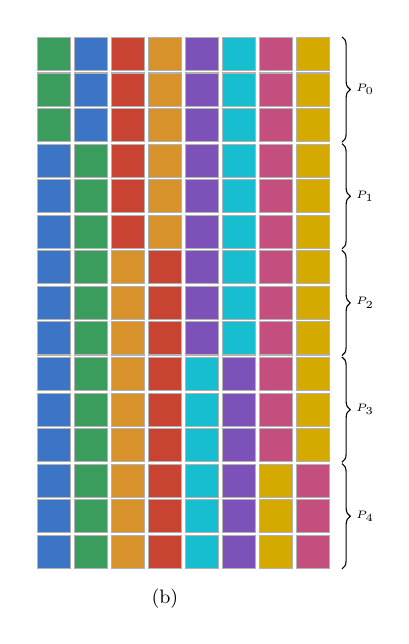
\begin{tikzpicture}[scale=0.78, transform shape]
\matrix (os) [matrix of nodes, nodes in empty cells,
  row sep=0.5pt, column sep=1pt,
  ampersand replacement=\&] {
|[n1]| \& |[n2]| \& |[n3]| \& |[n4]|
\& |[n5]| \& |[n6]| \& |[n7]| \& |[n8]| \\
|[n1]| \& |[n2]| \& |[n3]| \& |[n4]|
\& |[n5]| \& |[n6]| \& |[n7]| \& |[n8]| \\
|[n1]| \& |[n2]| \& |[n3]| \& |[n4]|
\& |[n5]| \& |[n6]| \& |[n7]| \& |[n8]| \\
|[n2]| \& |[n1]| \& |[n3]| \& |[n4]|
\& |[n5]| \& |[n6]| \& |[n7]| \& |[n8]| \\
|[n2]| \& |[n1]| \& |[n3]| \& |[n4]|
\& |[n5]| \& |[n6]| \& |[n7]| \& |[n8]| \\
|[n2]| \& |[n1]| \& |[n3]| \& |[n4]|
\& |[n5]| \& |[n6]| \& |[n7]| \& |[n8]| \\
|[n2]| \& |[n1]| \& |[n4]| \& |[n3]|
\& |[n5]| \& |[n6]| \& |[n7]| \& |[n8]| \\
|[n2]| \& |[n1]| \& |[n4]| \& |[n3]|
\& |[n5]| \& |[n6]| \& |[n7]| \& |[n8]| \\
|[n2]| \& |[n1]| \& |[n4]| \& |[n3]|
\& |[n5]| \& |[n6]| \& |[n7]| \& |[n8]| \\
|[n2]| \& |[n1]| \& |[n4]| \& |[n3]|
\& |[n6]| \& |[n5]| \& |[n7]| \& |[n8]| \\
|[n2]| \& |[n1]| \& |[n4]| \& |[n3]|
\& |[n6]| \& |[n5]| \& |[n7]| \& |[n8]| \\
|[n2]| \& |[n1]| \& |[n4]| \& |[n3]|
\& |[n6]| \& |[n5]| \& |[n7]| \& |[n8]| \\
|[n2]| \& |[n1]| \& |[n4]| \& |[n3]|
\& |[n6]| \& |[n5]| \& |[n8]| \& |[n7]| \\
|[n2]| \& |[n1]| \& |[n4]| \& |[n3]|
\& |[n6]| \& |[n5]| \& |[n8]| \& |[n7]| \\
|[n2]| \& |[n1]| \& |[n4]| \& |[n3]|
\& |[n6]| \& |[n5]| \& |[n8]| \& |[n7]| \\
};
\node[below=2mm] at (os-15-4.south) {\small (b)};
\draw[decorate,decoration={brace,amplitude=3pt}]
  ([xshift=2mm]os-1-8.north east)--
  ([xshift=2mm]os-3-8.south east)
  node[midway,right=3pt]{\tiny $P_0$};
\draw[decorate,decoration={brace,amplitude=3pt}]
  ([xshift=2mm]os-4-8.north east)--
  ([xshift=2mm]os-6-8.south east)
  node[midway,right=3pt]{\tiny $P_1$};
\draw[decorate,decoration={brace,amplitude=3pt}]
  ([xshift=2mm]os-7-8.north east)--
  ([xshift=2mm]os-9-8.south east)
  node[midway,right=3pt]{\tiny $P_2$};
\draw[decorate,decoration={brace,amplitude=3pt}]
  ([xshift=2mm]os-10-8.north east)--
  ([xshift=2mm]os-12-8.south east)
  node[midway,right=3pt]{\tiny $P_3$};
\draw[decorate,decoration={brace,amplitude=3pt}]
  ([xshift=2mm]os-13-8.north east)--
  ([xshift=2mm]os-15-8.south east)
  node[midway,right=3pt]{\tiny $P_4$};
\end{tikzpicture}
\caption{\textbf{Minimal music}: path from identity to the
paired-swap permutation $[2,1,4,3,6,5,8,7]$ via four
transpositions.
(a)~Bare path.
(b)~Ostinato rendering ($3\times$ repetition per state).}
\label{fig:minimal}
\end{figure}

Multiple targets can be concatenated into a cycle
$I\to\sigma_1\to\sigma_2\to\cdots\to\sigma_M\to I$,
yielding a periodic score with hierarchical structure.
The Cayley distance
$d_C(\sigma)=k-c(\sigma)$ (where $c$ counts cycles including
fixed points) provides a natural measure of the musical
\emph{duration} for each transformation.

%===================================================================
\section{Comparative overview}
\label{sec:compare}
%===================================================================

To explicitly synthesize the generative behaviors outlined in the preceding sections, Figure~\ref{fig:comparison} juxtaposes all four regimes in a single display.
The visual differences across the panels translate directly into their corresponding acoustic characteristics: the complete lack of vertical coherence in the white noise panel (a) yields a chaotic, saturated texture; the subtle, single-swap transitions in the brown noise panel (b) create a slow, drifting musical evolution; the Voss--McCartney multi-scale updates in the pink noise panel (c) balance recognizable structural continuity with sudden shifts; and the rigid, cumulative rank-2 transformations in the minimal music panel (d) visually capture the mechanical phase-shifting inherent in deterministic algorithms.

\begin{figure*}[t]
\centering
\setlength{\tabcolsep}{6pt}
\begin{tabular}{cccc}
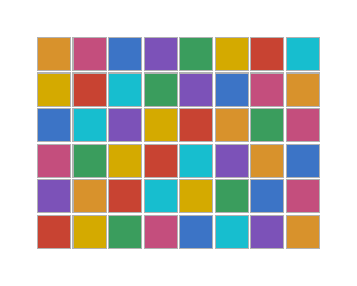
\begin{tikzpicture}[scale=0.78, transform shape]
\matrix (cw) [matrix of nodes, nodes in empty cells,
  row sep=0.5pt, column sep=0.5pt,
  ampersand replacement=\&] {
|[n4]| \& |[n7]| \& |[n2]| \& |[n5]|
\& |[n1]| \& |[n8]| \& |[n3]| \& |[n6]| \\
|[n8]| \& |[n3]| \& |[n6]| \& |[n1]|
\& |[n5]| \& |[n2]| \& |[n7]| \& |[n4]| \\
|[n2]| \& |[n6]| \& |[n5]| \& |[n8]|
\& |[n3]| \& |[n4]| \& |[n1]| \& |[n7]| \\
|[n7]| \& |[n1]| \& |[n8]| \& |[n3]|
\& |[n6]| \& |[n5]| \& |[n4]| \& |[n2]| \\
|[n5]| \& |[n4]| \& |[n3]| \& |[n6]|
\& |[n8]| \& |[n1]| \& |[n2]| \& |[n7]| \\
|[n3]| \& |[n8]| \& |[n1]| \& |[n7]|
\& |[n2]| \& |[n6]| \& |[n5]| \& |[n4]| \\
};
\end{tikzpicture}
&
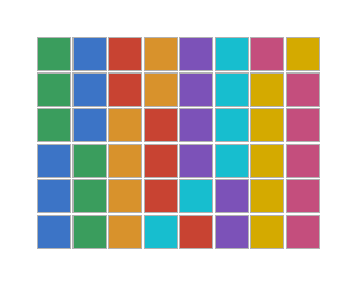
\begin{tikzpicture}[scale=0.78, transform shape]
\matrix (cb) [matrix of nodes, nodes in empty cells,
  row sep=0.5pt, column sep=0.5pt,
  ampersand replacement=\&] {
|[n1]| \& |[n2]| \& |[n3]| \& |[n4]|
\& |[n5]| \& |[n6]| \& |[n7]| \& |[n8]| \\
|[n1]| \& |[n2]| \& |[n3]| \& |[n4]|
\& |[n5]| \& |[n6]| \& |[n8]| \& |[n7]| \\
|[n1]| \& |[n2]| \& |[n4]| \& |[n3]|
\& |[n5]| \& |[n6]| \& |[n8]| \& |[n7]| \\
|[n2]| \& |[n1]| \& |[n4]| \& |[n3]|
\& |[n5]| \& |[n6]| \& |[n8]| \& |[n7]| \\
|[n2]| \& |[n1]| \& |[n4]| \& |[n3]|
\& |[n6]| \& |[n5]| \& |[n8]| \& |[n7]| \\
|[n2]| \& |[n1]| \& |[n4]| \& |[n6]|
\& |[n3]| \& |[n5]| \& |[n8]| \& |[n7]| \\
};
\end{tikzpicture}
&
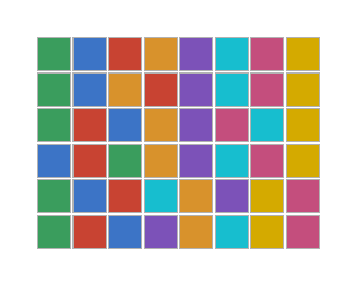
\begin{tikzpicture}[scale=0.78, transform shape]
\matrix (cp) [matrix of nodes, nodes in empty cells,
  row sep=0.5pt, column sep=0.5pt,
  ampersand replacement=\&] {
|[n1]| \& |[n2]| \& |[n3]| \& |[n4]|
\& |[n5]| \& |[n6]| \& |[n7]| \& |[n8]| \\
|[n1]| \& |[n2]| \& |[n4]| \& |[n3]|
\& |[n5]| \& |[n6]| \& |[n7]| \& |[n8]| \\
|[n1]| \& |[n3]| \& |[n2]| \& |[n4]|
\& |[n5]| \& |[n7]| \& |[n6]| \& |[n8]| \\
|[n2]| \& |[n3]| \& |[n1]| \& |[n4]|
\& |[n5]| \& |[n6]| \& |[n7]| \& |[n8]| \\
|[n1]| \& |[n2]| \& |[n3]| \& |[n6]|
\& |[n4]| \& |[n5]| \& |[n8]| \& |[n7]| \\
|[n1]| \& |[n3]| \& |[n2]| \& |[n5]|
\& |[n4]| \& |[n6]| \& |[n8]| \& |[n7]| \\
};
\end{tikzpicture}
&
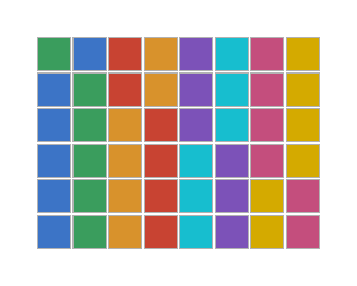
\begin{tikzpicture}[scale=0.78, transform shape]
\matrix (cm) [matrix of nodes, nodes in empty cells,
  row sep=0.5pt, column sep=0.5pt,
  ampersand replacement=\&] {
|[n1]| \& |[n2]| \& |[n3]| \& |[n4]|
\& |[n5]| \& |[n6]| \& |[n7]| \& |[n8]| \\
|[n2]| \& |[n1]| \& |[n3]| \& |[n4]|
\& |[n5]| \& |[n6]| \& |[n7]| \& |[n8]| \\
|[n2]| \& |[n1]| \& |[n4]| \& |[n3]|
\& |[n5]| \& |[n6]| \& |[n7]| \& |[n8]| \\
|[n2]| \& |[n1]| \& |[n4]| \& |[n3]|
\& |[n6]| \& |[n5]| \& |[n7]| \& |[n8]| \\
|[n2]| \& |[n1]| \& |[n4]| \& |[n3]|
\& |[n6]| \& |[n5]| \& |[n8]| \& |[n7]| \\
|[n2]| \& |[n1]| \& |[n4]| \& |[n3]|
\& |[n6]| \& |[n5]| \& |[n8]| \& |[n7]| \\
};
\end{tikzpicture}
\\
\small (a) White & \small (b) Brown &
\small (c) Pink  & \small (d) Minimal
\end{tabular}
\caption{Side-by-side comparison of six time steps
under the four regimes (all $k=8$).
(a)~White noise: no column coherence.
(b)~Brown noise: high local continuity.
(c)~Pink noise: multi-scale changes.
(d)~Minimal music: deterministic cumulative swaps.
Colors as in Fig.~\ref{fig:base}.}
\label{fig:comparison}
\end{figure*}

%===================================================================
\section{Prolog realization}
\label{sec:prolog}
%===================================================================

We implement all four regimes in
SWI-Prolog~\cite{swiprolog}, separating the structural layer
(permutation generation) from the rendering layer (MIDI pitch
assignment), following the SGLG framework
of~\cite{Jendreiko2025}.

The general SGLG for an $N$-step score is
\begin{align}
S &\to \mathrm{row}_1\;\mathrm{row}_2\;\cdots\;
       \mathrm{row}_N,
\label{eq:sglg-start}\\
\mathrm{row}_j &\to \mathrm{render}(P_j\mathbf{v}_C)\;br.
\label{eq:sglg-row}
\end{align}

\listingtitle{lst:core}{Core predicates: permutation
representation, Fisher--Yates shuffle, and swap.}
\begin{codeblock}
:- use_module(library(random)).
:- use_module(library(lists)).

identity(N, P) :- numlist(1, N, P).

% Fisher-Yates shuffle (white noise)
random_perm(N, P) :-
    identity(N, I),
    fisher_yates(I, P).
fisher_yates([], []).
fisher_yates(L, [H|T]) :-
    length(L, Len),
    random_between(1, Len, K),
    nth1(K, L, H),
    select(H, L, Rest),
    fisher_yates(Rest, T).

% Adjacent transposition
adj_swap(K, Pin, Pout) :-
    nth1(K, Pin, A), K1 is K+1,
    nth1(K1, Pin, B),
    set_nth(K, Pin, B, Tmp),
    set_nth(K1, Tmp, A, Pout).
set_nth(1,[_|T],X,[X|T]).
set_nth(N,[H|T],X,[H|R]) :-
    N>1, N1 is N-1,
    set_nth(N1,T,X,R).

% General swap
swap(I, J, Pin, Pout) :-
    nth1(I,Pin,A), nth1(J,Pin,B),
    set_nth(I,Pin,B,Tmp),
    set_nth(J,Tmp,A,Pout).
\end{codeblock}

\listingtitle{lst:regimes}{Brown, pink, and minimal-music
generators.}
\begin{codeblock}
% Brown noise: random walk
brown_step(N, Pin, Pout) :-
    Max is N-1,
    random_between(1, Max, K),
    adj_swap(K, Pin, Pout).
brown_seq(_, P, 0, [P]).
brown_seq(N, P, S, [P|R]) :-
    S>0, brown_step(N,P,P1),
    S1 is S-1, brown_seq(N,P1,S1,R).

% Pink noise (Voss-McCartney)
pink_step(T, N, Rs0, Rs1, Perm) :-
    update_regs(T, 0, N, Rs0, Rs1),
    identity(N, Id),
    compose_regs(Rs1, Id, Perm).
update_regs(_, _, _, [], []).
update_regs(T, K, N, [R|Rs],[R1|Rs1]):-
    B is (T>>K)/\ 1,
    P is ((T-1)>>K)/\ 1,
    (B=\=P -> rand_adj(N,R1) ; R1=R),
    K1 is K+1,
    update_regs(T,K1,N,Rs,Rs1).
rand_adj(N, swap(A,B)) :-
    Max is N-1,
    random_between(1,Max,A), B is A+1.
compose_regs([], P, P).
compose_regs([swap(A,B)|Rs], Pin, Po):-
    swap(A, B, Pin, P1),
    compose_regs(Rs, P1, Po).

% Minimal music: decompose into swaps
minimal_path(P, P, []).
minimal_path(Cur, Tgt, [swap(I,J)|Ss]):-
    Cur \= Tgt,
    first_diff(Cur, Tgt, 1, I),
    nth1(I, Tgt, V),
    nth1(J, Cur, V),
    swap(I, J, Cur, Next),
    minimal_path(Next, Tgt, Ss).
first_diff([H|_],[H2|_],K,K):- H=\=H2,!.
first_diff([_|A],[_|B],K,R):-
    K1 is K+1, first_diff(A,B,K1,R).
\end{codeblock}

\listingtitle{lst:render}{Rendering layer and DCG output.}
\begin{codeblock}
% Map to MIDI pitch (C major scale)
pitch(Deg, Midi) :-
    Scale=[0,2,4,5,7,9,11,12],
    D1 is Deg-1, nth0(D1,Scale,Off),
    Midi is 60 + Off.

% DCG rendering
render([]) --> [].
render([H|T]) --> note(H), render(T).
note(1)-->[c4].  note(2)-->[d4].
note(3)-->[e4].  note(4)-->[f4].
note(5)-->[g4].  note(6)-->[a4].
note(7)-->[b4].  note(8)-->[c5].
br --> [rest].

% Main entry points
play_white(N, Steps) :-
    forall(between(1,Steps,_),
      (random_perm(N,P),
       phrase(render(P),Out),
       writeln(Out))).

play_minimal(N, Target) :-
    identity(N, Id),
    minimal_path(Id, Target, Swaps),
    replay(Id, Swaps).
replay(P, []) :-
    phrase(render(P),Out), writeln(Out).
replay(P, [swap(I,J)|Ss]) :-
    phrase((render(P),br),Out),
    writeln(Out),
    swap(I,J,P,P1), replay(P1,Ss).
\end{codeblock}

The output of \texttt{play\_minimal(8, [2,1,4,3,6,5,8,7])}
produces exactly the five-row terminal sequence depicted in
Fig.~\ref{fig:minimal}(a).
When this list of terminal symbols is passed to a MIDI engine
or via OSC to a synthesizer, the algebraic path becomes an
audible score.

%===================================================================
\section{Discussion}
\label{sec:discussion}
%===================================================================

\subsection{The unitary--permutation bridge}

The hierarchy $S_k\subset O(k)\subset U(k)$ is not merely a
mathematical observation; it has direct generative
consequences.
Every regime defined in this paper---white, brown, pink,
minimal---has a continuous counterpart on $O(k)$ or $U(k)$.
White noise on $S_k$ corresponds to Haar-random sampling on
$U(k)$~\cite{mezzadri-07}.
Brown noise corresponds to Brownian motion on the Lie
group~\cite{liao-04}.
The minimal-music decomposition into transpositions
corresponds to factoring a unitary into Givens rotations or
two-level unitaries~\cite{nielsen-chuang-00,golub-vanloan-13}.

Working with permutations rather than continuous matrices
offers two practical advantages.
First, the output at each time step is a \emph{deterministic
reassignment} of the $k$ voices---no superpositions, no
fractional amplitudes---which maps directly to the
combinatorial constraints of traditional polyphonic writing.
Second, the finite group $S_k$ is exactly enumerable and
implementable in a logic-programming language without
floating-point arithmetic.

At the same time, the unitary perspective suggests natural
extensions.
One could interpolate between two permutation matrices via a
geodesic on $O(k)$ or $U(k)$, producing a continuous
``crossfade'' between two discrete voice assignments.
Such interpolations would introduce the relative phases and
superpositions characteristic of quantum mechanics into the
generative framework.

\subsection{Structure as constraint}

In classical generative art, random noise is often applied
directly to synthesis parameters.
In our method, randomness operates on the \emph{syntactic
skeleton}---the permutation matrix.
The result is a composition that never violates the set
constraints: no matter how chaotic a white-noise permutation
becomes, the output row contains exactly all $k$ notes without
duplication.
The algebraic properties of the permutation matrix act as an
unbreakable conservation law for the musical material.

\subsection{Perceptual offerings and time}

When we compare the partition-logic visual artifacts of
Ref.~\cite{jendreiko-svozil-2026} with the permutation-based
musical scores generated here, the crucial variable is
\emph{time}.
A visual grammar presents its entire derivation
simultaneously; a musical grammar is a \emph{temporal
perceptual offering}.
The brown-noise sequences afford acts of auditory
tracking---the listener can hear the rank-2 transpositions
bubbling through the sequence.
The minimal-music trajectories afford a sense of geometric
convergence, building tension as the vector is slowly sorted
into the target permutation.

\subsection{Generalization}

The construction generalizes immediately from $k=8$ to
arbitrary rank.
Larger~$k$ yields denser pitch fields and longer minimal paths;
smaller~$k$ produces sparser, more audibly transparent
textures.
The same permutation sequence can be rendered as pitch
assignments, rhythmic patterns, spatial positions, or timbral
interpolations by changing only the rendering predicates.

\subsection{Connection to Hauer's \emph{Zw\"olftonspiel}}
\label{sec:hauer}

The permutation-based framework developed in this paper has a
significant historical precedent in the work of the Austrian
composer Josef Matthias Hauer
(1883--1959)~\cite{hauer-25,hauer-26,sengstschmid-80}.
Hauer developed his twelve-tone method independently of---and
slightly prior to---Arnold
Schoenberg~\cite{schoenberg-75,wille-76}, but his approach is
arguably more purely permutational and therefore closer in
spirit to the present work.

\subsubsection{Hauer's system as permutation music}

In Hauer's \emph{Zw\"olftonspiel} (literally: twelve-tone game
or play), the chromatic aggregate $\Omega_{12}=\{0,1,\ldots,11\}$
of twelve pitch classes is the primary material.
A twelve-tone row is a permutation $\sigma\in S_{12}$ of this
set: every pitch class appears exactly once, and the
compositional act consists in choosing and ordering these
permutations.
This is precisely the framework of the present paper,
specialized to $k=12$ and the chromatic rather than diatonic
scale.

The constraint that every row is a \emph{complete} permutation
of all $k$ pitch classes---no omissions, no
repetitions---functions in both Hauer's system and in our
framework as an ``unbreakable conservation law'' for the
musical material.
In our language (Sec.~\ref{sec:discussion}), the doubly
stochastic property of the permutation matrix guarantees this
conservation at every time step.

\subsubsection{Tropes as equivalence classes on $S_{12}$}

Hauer's most distinctive contribution is the concept of the
\emph{Trope} (trope)~\cite{hauer-25,sengstschmid-80}.
He partitions the twelve pitch classes into two complementary
\emph{hexachords} (sets of six), disregarding the internal
ordering within each half.
Two such partitions are considered equivalent if one can be
obtained from the other by transposition
(cyclic shift in $\mathbb{Z}_{12}$).

In group-theoretic terms, a trope is an orbit of the action
of $\mathbb{Z}_{12}$ on the set of unordered complementary
hexachord pairs:
\begin{equation}
\mathcal{T} = \left\{\{H,\,\Omega_{12}\setminus H\}
\;\Big|\; H\subset\Omega_{12},\;|H|=6\right\}
\Big/ \mathbb{Z}_{12}.
\label{eq:tropes}
\end{equation}
Hauer identified exactly $44$ such trope
classes~\cite{hauer-26,sengstschmid-80,haluska-04}, a count
that can be verified by Burnside's
lemma~\cite{burnside-1897}.

Within each trope, the internal ordering of the two hexachords
is free---that is, any element of $S_6\times S_6$ may be
applied independently to the two halves.
The trope therefore acts as a \emph{macro-structural
constraint} (which six pitches go together), while the
micro-structure (the ordering within each hexachord) provides
a space of $(6!)^2 = 518\,400$ possible realizations per
trope.

This two-level architecture---a coarse partition into tropes,
followed by free permutation within each half---is a
precursor of the three-layer separation (formal skeleton,
generative grammar, rendering map) advocated in
Refs.~\cite{jendreiko-svozil-2026,Jendreiko2025} and employed
throughout the present paper.

\subsubsection{Hauer versus Schoenberg}

It is instructive to contrast Hauer's approach with
Schoenberg's better-known twelve-tone
technique~\cite{schoenberg-75}.
Schoenberg fixes a single \emph{tone row} (a specific
permutation $\sigma_0\in S_{12}$) and derives all subsequent
material from it by four operations: identity,
retrograde~$R$, inversion~$I$, and retrograde
inversion~$RI$, each combined with the twelve
transpositions~$T_n$.
This yields a group of exactly $48$ row forms---a small
subgroup of~$S_{12}$.

Hauer, by contrast, does not privilege a single row.
His \emph{Spiel} (game) character allows free navigation
within the vast space of $12!=479\,001\,600$ permutations,
subject only to the trope constraint.
In the terminology of this paper, Schoenberg's method is a
\emph{minimal-music regime} (a small, deterministic set of
transformations applied to a fixed starting point), whereas
Hauer's method is closer to a \emph{constrained random walk}
on $S_{12}$, with the trope acting as a hyperplane constraint
that restricts the walk to a subset of the Cayley graph.

Table~\ref{tab:hauer} summarizes the comparison.

\begin{table}[t]
\caption{Comparison of Hauer's \emph{Zw\"olftonspiel},
Schoenberg's twelve-tone method, and the present framework.
All three operate on a symmetric group $S_k$ but differ in the
constraints and traversal strategies applied.}
\label{tab:hauer}
\begin{ruledtabular}
\begin{tabular}{lccc}
 & Hauer & Schoenberg & This paper \\
\hline
$k$ & 12 & 12 & arbitrary \\
Constraint & trope & fixed row & none / adj.\ \\
Row forms & $(6!)^2$ & $\le 48$ & $k!$ \\
Traversal & free & deterministic & white/brown/ \\
 & & & pink/minimal \\
Transformation group & $\mathbb{Z}_{12}$ (trope level) & $D_{12}\!\times\!\mathbb{Z}_2$ & $S_k$ \\
\end{tabular}
\end{ruledtabular}
\end{table}

\subsubsection{Hauer's tropes and noise regimes}

The connection between Hauer's tropes and our noise regimes is
suggestive.
A \emph{white-noise Zw\"olftonspiel} would draw each successive
row uniformly at random from the $518\,400$ permutations
compatible with a given trope---a constrained version of our
white-noise regime (Sec.~\ref{sec:white}).
A \emph{brown-noise Zw\"olftonspiel} would perform a random walk
on the Cayley graph of $S_6\times S_6$ within the trope,
applying adjacent transpositions independently to the two
hexachords---producing the slowly drifting texture of
Sec.~\ref{sec:brown}, but with the added structural feature
that the hexachord boundary is never crossed.
A \emph{minimal-music Zw\"olftonspiel} would reach a target
permutation within the trope by a sequence of at most $10$
transpositions (at most $5$ per hexachord), yielding a
Reich-like phasing process on the chromatic aggregate.

These constructions suggest that Hauer's trope system can be
naturally embedded within our generative framework by
restricting the permutation group from $S_{12}$ to
$S_6\times S_6$ (or, more precisely, to the coset of
$S_6\times S_6$ in $S_{12}$ defined by the trope).

\subsubsection{The \emph{Spiel} as generative grammar}

Finally, Hauer's deliberate use of the word \emph{Spiel}
(game, play) for his compositional method resonates with the
generative-logic perspective of Jendreiko's
SGLGs~\cite{Jendreiko2024,Jendreiko2025}.
In both cases, the compositional act is framed not as the
expression of subjective intention but as the disciplined
exploration of a combinatorial space defined by explicit rules.
The composer does not ``write'' the music; rather, the
composer \emph{sets up the game} and lets the rules
generate the material.
This is precisely the ethos of Generative Logic applied to
sonic production.

Hauer's work thus appears, in retrospect, as an early
instance of permutation-based generative composition---a
practice that the present paper formalizes, generalizes, and
implements in executable logic-programming form.


%===================================================================
\section{Conclusion}
\label{sec:conclusion}
%===================================================================

We have demonstrated that sequences of finite permutation
matrices---the binary distillation of unitary quantum
evolution---serve as powerful structural engines for generative
logic programming and algorithmic composition.
The group-theoretic hierarchy
$S_k\subset O(k)\subset U(k)$ situates our constructions
within the broader landscape of quantum-mechanical
transformations: permutation matrices retain the essential
properties of unitarity (invertibility, norm preservation,
one-to-one basis mapping) while restricting all entries to
$\{0,1\}$.

By mapping the identity matrix to a base musical vector, we
translate paths on the Cayley graph of~$S_k$ into perceptible
sonic experiences.
We formulated three stochastic
regimes---white, brown, and pink noise---and one deterministic
regime inspired by minimal music, each with a well-defined
continuous analogue on $O(k)$ or $U(k)$.

We have also shown that the framework naturally subsumes
Hauer's \emph{Zw\"olftonspiel} as the special case $k=12$
with a trope constraint restricting the permutation group to
$S_6\times S_6$, thereby connecting early twentieth-century
twelve-tone practice to contemporary logic programming and
noise-theoretic models.

Through Prolog-based SGLGs, the matrix arithmetic is
formalized as an executable logic grammar, explicitly isolating
the mathematical skeleton from the acoustic rendering.
The permutation matrix is transformed from a dry algebraic
operator into an expressive, generative score.

\begin{acknowledgments}
Christian Jendreiko would like to thank Fran\c{c}ois Fages,
Thierry Marianne, and Guy Narboni for the invaluable insights
gained during a collaborative working session in Paris.
This research was funded in whole or in part by the
\textit{Austrian Science Fund (FWF)}
[Grant \textit{DOI:10.55776/PIN5424624}].
The authors acknowledge TU Wien Bibliothek for financial
support through its Open Access Funding Programme.
\end{acknowledgments}

\begin{thebibliography}{20}

\bibitem{jendreiko-svozil-2026}
C.~Jendreiko and K.~Svozil,
Quantum structures as generative scores:
Partition logic, Generative Logic, and aesthetic form,
arXiv:2503.15654 [quant-ph] (2025).

\bibitem{Jendreiko2024}
C.~Jendreiko,
Generative logic: Teaching Prolog as generative AI in art and
design,
in \emph{Workshop Proceedings of the 40th International
Conference on Logic Programming (ICLP-WS 2024)},
CEUR Workshop Proceedings, Vol.~3799,
edited by J.~Arias \emph{et al.}
(CEUR-WS.org, Dallas, TX, 2024).

\bibitem{Jendreiko2025}
C.~Jendreiko,
The simple generative logic grammar: A tool for teaching
logical thinking through visual research in art and design,
in \emph{Joint Proceedings of the Workshops and Doctoral
Consortium of the 41st International Conference on Logic
Programming (ICLP-WS-DC 2025)},
CEUR Workshop Proceedings, Vol.~4117,
edited by D.~Azzolini \emph{et al.}
(CEUR-WS.org, Rende, 2025).

\bibitem{vonneumann-32}
J.~von Neumann,
\emph{Mathematische Grundlagen der Quantenmechanik}
(Springer, Berlin, 1932);
English translation: \emph{Mathematical Foundations of Quantum
Mechanics} (Princeton University Press, Princeton, 1955).

\bibitem{peres-93}
A.~Peres,
\emph{Quantum Theory: Concepts and Methods}
(Kluwer, Dordrecht, 1993).

\bibitem{hall-15}
B.~C. Hall,
\emph{Lie Groups, Lie Algebras, and Representations},
2nd~ed.\ (Springer, Cham, 2015).

\bibitem{nielsen-chuang-00}
M.~A. Nielsen and I.~L. Chuang,
\emph{Quantum Computation and Quantum Information}
(Cambridge University Press, Cambridge, 2000).

\bibitem{birkhoff-46}
G.~Birkhoff,
Three observations on linear algebra,
Univ.\ Nac.\ Tucum\'an Rev.\ Ser.~A \textbf{5}, 147 (1946).

\bibitem{schur-23}
I.~Schur,
\"Uber eine Klasse von Mittelbildungen mit Anwendungen auf
die Determinantentheorie,
Sitzungsber.\ Berl.\ Math.\ Ges.\ \textbf{22}, 9 (1923).

\bibitem{horn-54}
A.~Horn,
Doubly stochastic matrices and the diagonal of a rotation
matrix,
Am.\ J.\ Math.\ \textbf{76}, 620 (1954).

\bibitem{golub-vanloan-13}
G.~H. Golub and C.~F. Van~Loan,
\emph{Matrix Computations}, 4th~ed.\
(Johns Hopkins University Press, Baltimore, 2013).

\bibitem{liao-04}
M.~Liao,
\emph{L\'evy Processes in Lie Groups}
(Cambridge University Press, Cambridge, 2004).

\bibitem{mezzadri-07}
F.~Mezzadri,
How to generate random matrices from the classical compact
groups,
Notices Am.\ Math.\ Soc.\ \textbf{54}, 592 (2007).

\bibitem{swiprolog}
J.~Wielemaker, T.~Schrijvers, M.~Triska, and T.~Lager,
{SWI-Prolog},
Theory and Practice of Logic Programming \textbf{12}, 67
(2012).

\bibitem{knuth-97}
D.~E. Knuth,
\emph{The Art of Computer Programming},
Vol.~2: Seminumerical Algorithms, 3rd~ed.
(Addison-Wesley, Reading, MA, 1997).

\bibitem{xenakis-71}
I.~Xenakis,
\emph{Formalized Music}
(Indiana University Press, Bloomington, 1971).

\bibitem{diaconis-shahshahani-81}
P.~Diaconis and M.~Shahshahani,
Generating a random permutation with random transpositions,
Z.\ Wahrscheinlichkeitstheorie verw.\ Gebiete \textbf{57},
159 (1981).

\bibitem{voss-clarke-75}
R.~F. Voss and J.~Clarke,
``$1/f$ noise'' in music and speech,
Nature \textbf{258}, 317 (1975).

\bibitem{voss-clarke-78}
R.~F. Voss and J.~Clarke,
``$1/f$ noise'' in music: Music from $1/f$ noise,
J.\ Acoust.\ Soc.\ Am.\ \textbf{63}, 258 (1978).

\bibitem{gardner-78}
M.~Gardner,
White and brown music, fractal curves and one-over-$f$
fluctuations,
Sci.\ Am.\ \textbf{238}(4), 16 (1978).

\bibitem{hauer-25}
J.~M. Hauer,
\emph{Vom Melos zur Pauke: Eine Einf\"uhrung in die
Zw\"olftonmusik}
(Universal Edition, Vienna, 1925).

\bibitem{hauer-26}
J.~M. Hauer,
\emph{Zw\"olftontechnik: Die Lehre von den Tropen}
(Universal Edition, Vienna, 1926).

\bibitem{sengstschmid-80}
J.~Sengstschmid,
\emph{Zwischen Trope und Zw\"olftonspiel:
J.~M. Hauers Zw\"olftonmusik}
(Bosse, Regensburg, 1980).

\bibitem{haluska-04}
J.~Halu\v{s}ka,
\emph{The Mathematical Theory of Tone Systems}
(Marcel Dekker, New York, 2004).

\bibitem{schoenberg-75}
A.~Schoenberg,
\emph{Style and Idea: Selected Writings},
edited by L.~Stein
(Faber \& Faber, London, 1975).

\bibitem{wille-76}
R.~Wille,
Mathematik und Musiktheorie,
in \emph{Musik und Zahl},
edited by G.~Schnitzler
(Verlag f\"ur systematische Musikwissenschaft, Bonn, 1976),
pp.~233--264.

\bibitem{burnside-1897}
W.~Burnside,
\emph{Theory of Groups of Finite Order}
(Cambridge University Press, Cambridge, 1897);
2nd~ed.\ (1911; reprinted Dover, New York, 1955).

\end{thebibliography}

\end{document}
